% ABOUTME: Main document of the IEEE conference report for the 5-stage pipelined RISC-V project.
% ABOUTME: Title, authors and abstract; every section is a fragment under sections/.
\documentclass[conference]{IEEEtran}
\usepackage{graphicx}
\usepackage{amsmath}
\usepackage{cite}
\usepackage{booktabs}
\usepackage{listings}
\graphicspath{{../figures/}}
\lstset{basicstyle=\ttfamily\footnotesize, columns=fullflexible, frame=single}

\begin{document}

\title{A Five-Stage Pipelined RISC-V Processor: Design, Verification and the Measured Cost of Hazards}

\author{\IEEEauthorblockN{Sarvesh Srinath, Trishit Swarnakar, Aryan Kumar,
Husain Khorakiwala and Navodit Sharma}
\IEEEauthorblockA{Modern Computer Architecture, Verilog Project 3}}

\maketitle

\begin{abstract}
We design a single-cycle processor for an 18 instruction subset of RV32I in
Verilog, verify it, and partition the same datapath into the classic
five-stage pipeline (IF, ID, EX, MEM, WB) with pipeline registers, a hazard
unit and a forwarding unit. Every design is checked against a Python
instruction set simulator on 11 directed hazard tests, 5 benchmarks and 40
constrained-random programs, 248 automated checks in all. On a Lattice ECP5
FPGA the pipeline raises the maximum clock from 58.8 MHz to 113.9 MHz
without forwarding and to 83.9 MHz with it. Without forwarding, CPI ranges
from 1.51 to 2.74; forwarding removes every arithmetic stall and brings CPI to
1.26 to 1.58. Because every taken branch costs two cycles and our loops end
in one, the net execution time speedup over the single-cycle design is
0.90 to 1.14 with forwarding and 0.71 to 1.29 without. The iron law of
performance explains every result: with forwarding the pipeline wins only
when its CPI stays below the clock ratio of 1.43. We trace each lost cycle
to its cause and each nanosecond of the critical path to its stage.
\end{abstract}

\begin{IEEEkeywords}
RISC-V, pipelining, hazards, forwarding, CPI, FPGA, Verilog
\end{IEEEkeywords}

% ABOUTME: Introduction: why pipeline a processor, what we built, what we contribute and the paper's layout.
% ABOUTME: Owner: Navodit. Numbers are from results/.
\section{Introduction}
\label{sec:intro}

A single-cycle processor completes every instruction in one clock cycle, so
the clock period has to fit the slowest instruction: fetch, register read,
ALU, data memory and write back, one after another. Pipelining cuts this path
into stages with registers between them. Several instructions are then in
flight at once, and each cycle only has to cover one stage, so the clock can
run faster. The cost is hazards: an instruction may need a result that an
older instruction has not written yet, or the processor may fetch the wrong
instructions after a branch \cite{patterson2021}.

In the ideal case a five-stage pipeline is five times faster. This project
asks how much of that gain survives in a real design on real hardware. We
built three processors for the same RV32I subset \cite{riscvspec}: a
single-cycle baseline, a five-stage pipeline that stalls on every data
hazard, and the same pipeline with forwarding. All three were verified
against the same reference model, synthesised for the same FPGA and run on
the same benchmarks, so any difference between them comes from the
microarchitecture alone.

Our contributions are:
\begin{itemize}
\item a single-cycle CPU and a five-stage pipelined CPU in Verilog, with one
module per stage and per pipeline register;
\item a verification flow that compares every register and memory word with a
Python instruction set simulator, on directed hazard tests, benchmarks and
constrained-random programs (248 checks);
\item cycle accurate performance counters and pipeline diagrams drawn from the
hardware's own trace;
\item synthesis and place and route results on a Lattice ECP5 FPGA, with the
critical path of each design explained stage by stage;
\item a CPI, IPC and execution time comparison that separates the gain from a
shorter clock from the losses to pipeline fill, stalls and branch flushes.
\end{itemize}

Section~\ref{sec:background} reviews related work and the performance model.
Sections~\ref{sec:single} and~\ref{sec:pipeline} describe the two designs,
Section~\ref{sec:verification} how we verified them and
Section~\ref{sec:results} what we measured. Section~\ref{sec:conclusion}
concludes and sets out the Phase II plan.
% ABOUTME: Literature review (prior pipelines, open RISC-V cores, branch handling) and background.
% ABOUTME: Owner: Navodit. Background covers CPI, IPC, the iron law and the three kinds of hazard.
\section{Literature Review and Background}
\label{sec:background}

\subsection{Pipelined processors}
The Stanford MIPS processor \cite{hennessy1982} showed that a simple
load/store instruction set lets a single chip run a deep pipeline at a high
clock. MIPS left hazards to the compiler, which had to schedule instructions
so that no result was used too early. Later designs, including ours, detect
hazards in hardware instead. The five-stage pipeline we build (IF, ID, EX,
MEM, WB) is the one Patterson and Hennessy use to teach pipelining
\cite{patterson2021}, together with the forwarding unit, the load-use stall
and the branch flush. Hennessy and Patterson \cite{hennessy2019} give the
iron law of performance that we use to explain every result.

\subsection{RISC-V and open-source cores}
RISC-V is a free and open instruction set from UC Berkeley. Asanovi\'c and
Patterson \cite{asanovic2014} argue that a free ISA lets anyone build and
share implementations without a licence, and that a simple RISC design is the
right base for one. Open RISC-V cores now cover a wide range of designs.
PicoRV32 \cite{picorv32} is optimised for size and clock speed, not
throughput: it takes several cycles per instruction (an average CPI of about
4.2 on Dhrystone). Ibex \cite{ibex} has a two-stage pipeline, fetch and a
combined decode and execute stage. Rocket \cite{rocketchip} is a five-stage
in-order core like ours, with caches and branch prediction, and has been
manufactured and has booted Linux. Our design is the same five stages as
Rocket with none of those extras, so the cost of each hazard can be measured
on its own.

\subsection{Branch handling}
Smith \cite{smith1981} compared branch prediction strategies and showed that
dynamic prediction, which learns from each branch's history, beats fixed
rules. We use the simplest fixed rule, predict not taken, and Section
\ref{sec:results} measures what it costs. That cost is the starting point for
our Phase II work.

\subsection{Performance measures}
For a program of $N$ instructions that takes $C$ clock cycles at clock
frequency $f$,
\begin{equation}
\mathrm{CPI} = \frac{C}{N}, \qquad \mathrm{IPC} = \frac{N}{C}, \qquad
T = \frac{N \cdot \mathrm{CPI}}{f}.
\label{eq:ironlaw}
\end{equation}
The last expression is the iron law of processor performance
\cite{hennessy2019}. Throughput is $f \cdot \mathrm{IPC}$ instructions per
second. A single-cycle CPU has $\mathrm{CPI}=1$ exactly; a pipeline aims for
CPI close to 1 at a much higher $f$.

For the same program, the speedup of a pipeline over the single-cycle design
follows from (\ref{eq:ironlaw}):
\begin{equation}
S = \frac{T_{\text{single}}}{T_{\text{pipe}}} =
\frac{f_{\text{pipe}} / f_{\text{single}}}{\mathrm{CPI}_{\text{pipe}}}.
\label{eq:speedup}
\end{equation}
The pipeline is faster only when its CPI is below its clock ratio.

\subsection{Pipeline cycle accounting}
A five-stage pipeline needs four cycles to fill before the first instruction
completes. After that, every lost cycle has one of two causes in our design:
a stall, where the instruction in ID waits for an operand, or a flush, where
a taken branch discards the two younger instructions already fetched. So
\begin{equation}
C = N + 4 + \text{stalls} + 2 \cdot \text{taken branches}.
\label{eq:cycles}
\end{equation}
Our test suite checks this identity on every directed program and benchmark in both pipeline modes.

\subsection{Hazards}
\emph{Structural hazards} arise when two stages need one resource. Separate
instruction and data memories (a Harvard layout) and a register file with two
read ports and one write port remove them.
\emph{Data hazards} arise when an instruction reads a register that an older
instruction has not yet written. A pipeline either stalls until the value is
in the register file, or forwards it from a later pipeline register straight
to the ALU inputs. A load is the exception: its data only exists after MEM,
so a use in the very next instruction must wait one cycle even with
forwarding (the load-use hazard).
\emph{Control hazards} arise because the next PC after a branch is known only
when the branch resolves. We predict not taken and resolve branches in EX, so
each taken branch costs two cycles.

% ABOUTME: The instruction subset and the single-cycle datapath and control unit.
% ABOUTME: Owner: Aryan (review against rtl/common and rtl/single_cycle, then defend in viva).
\section{Instruction Set and Single-Cycle Design}
\label{sec:single}

\subsection{Instruction subset}
The brief suggests ADD, SUB, ADDI, LW, SW, BEQ and BNE. We add the logic,
compare and shift instructions needed for realistic benchmarks such as
sorting, 18 instructions in all (Table~\ref{tab:isa}). Memory accesses are
aligned 32 bit words. \texttt{ecall} marks the end of a program.

\begin{table}[t]
\centering
\caption{Supported RV32I instructions}
\label{tab:isa}
\begin{tabular}{@{}ll@{}}
\toprule
Format & Instructions \\
\midrule
R & \texttt{add sub and or xor slt sll} \\
I & \texttt{addi andi ori xori slti slli} \\
I (load), S & \texttt{lw}, \texttt{sw} \\
B & \texttt{beq bne} \\
System & \texttt{ecall} (halt) \\
\bottomrule
\end{tabular}
\end{table}

\subsection{Datapath}
The datapath is built from shared modules in \texttt{rtl/common}: a 32 bit
ALU with seven operations, a $32\times32$ register file with two
asynchronous read ports and one synchronous write port (x0 always reads
zero), an immediate generator for the I, S and B formats, and two 256 word
memories. In the single-cycle CPU (\texttt{cpu\_single.v}) one instruction
passes through all of them in one clock period: the PC addresses instruction
memory, the fields address the register file, the ALU computes a result or an
address, data memory is read or written, and the write-back mux returns the
ALU result or the loaded word to the register file. A taken branch loads
$\mathrm{PC}+\mathrm{imm}$ instead of $\mathrm{PC}+4$.

\subsection{Control unit}
The control unit (\texttt{control.v}) decodes the opcode, \texttt{funct3}
and \texttt{funct7} into the signals of Table~\ref{tab:control}. It also
reports whether the instruction really reads \texttt{rs1} and \texttt{rs2}.
In an I-type instruction the \texttt{rs2} field holds immediate bits, and
without this flag the pipeline's hazard unit would stall on registers the
instruction never reads.

\begin{table}[t]
\centering
\caption{Main control signals per instruction class}
\label{tab:control}
\small
\setlength{\tabcolsep}{3pt}
\begin{tabular}{@{}lcccccc@{}}
\toprule
Class & RegWr & ALUSrc & MemRd & MemWr & Br & ALU \\
\midrule
R-type & 1 & reg & 0 & 0 & 0 & funct \\
I-type & 1 & imm & 0 & 0 & 0 & funct3 \\
\texttt{lw} & 1 & imm & 1 & 0 & 0 & add \\
\texttt{sw} & 0 & imm & 0 & 1 & 0 & add \\
\texttt{beq}/\texttt{bne} & 0 & reg & 0 & 0 & 1 & compare \\
\bottomrule
\end{tabular}
\end{table}

\subsection{Critical path}
Place and route on the ECP5 (Section~\ref{sec:results}) reports a longest
path of 17.0\,ns, or 58.75\,MHz. Because the instruction memory is a ROM built
from logic, Yosys moves the PC register to the ROM's output, so the path starts
with the instruction already in flip-flops. From there it runs through a
register file read (2.1\,ns), the ALU computing the address (3.2\,ns), a read of
the 256 word data memory (8.0\,ns, the largest share) and the write-back mux to
the register file's write port (3.2\,ns, plus setup). Every instruction pays
for this path, even an \texttt{addi} that never touches data memory.

% ABOUTME: The five-stage pipeline: partitioning, pipeline registers, hazard and forwarding units.
% ABOUTME: Owner: Sarvesh (with Aryan for the datapath and control partitioning).
\section{Proposed Solution: Five-Stage Pipeline}
\label{sec:pipeline}

\begin{figure*}[t]
\centering
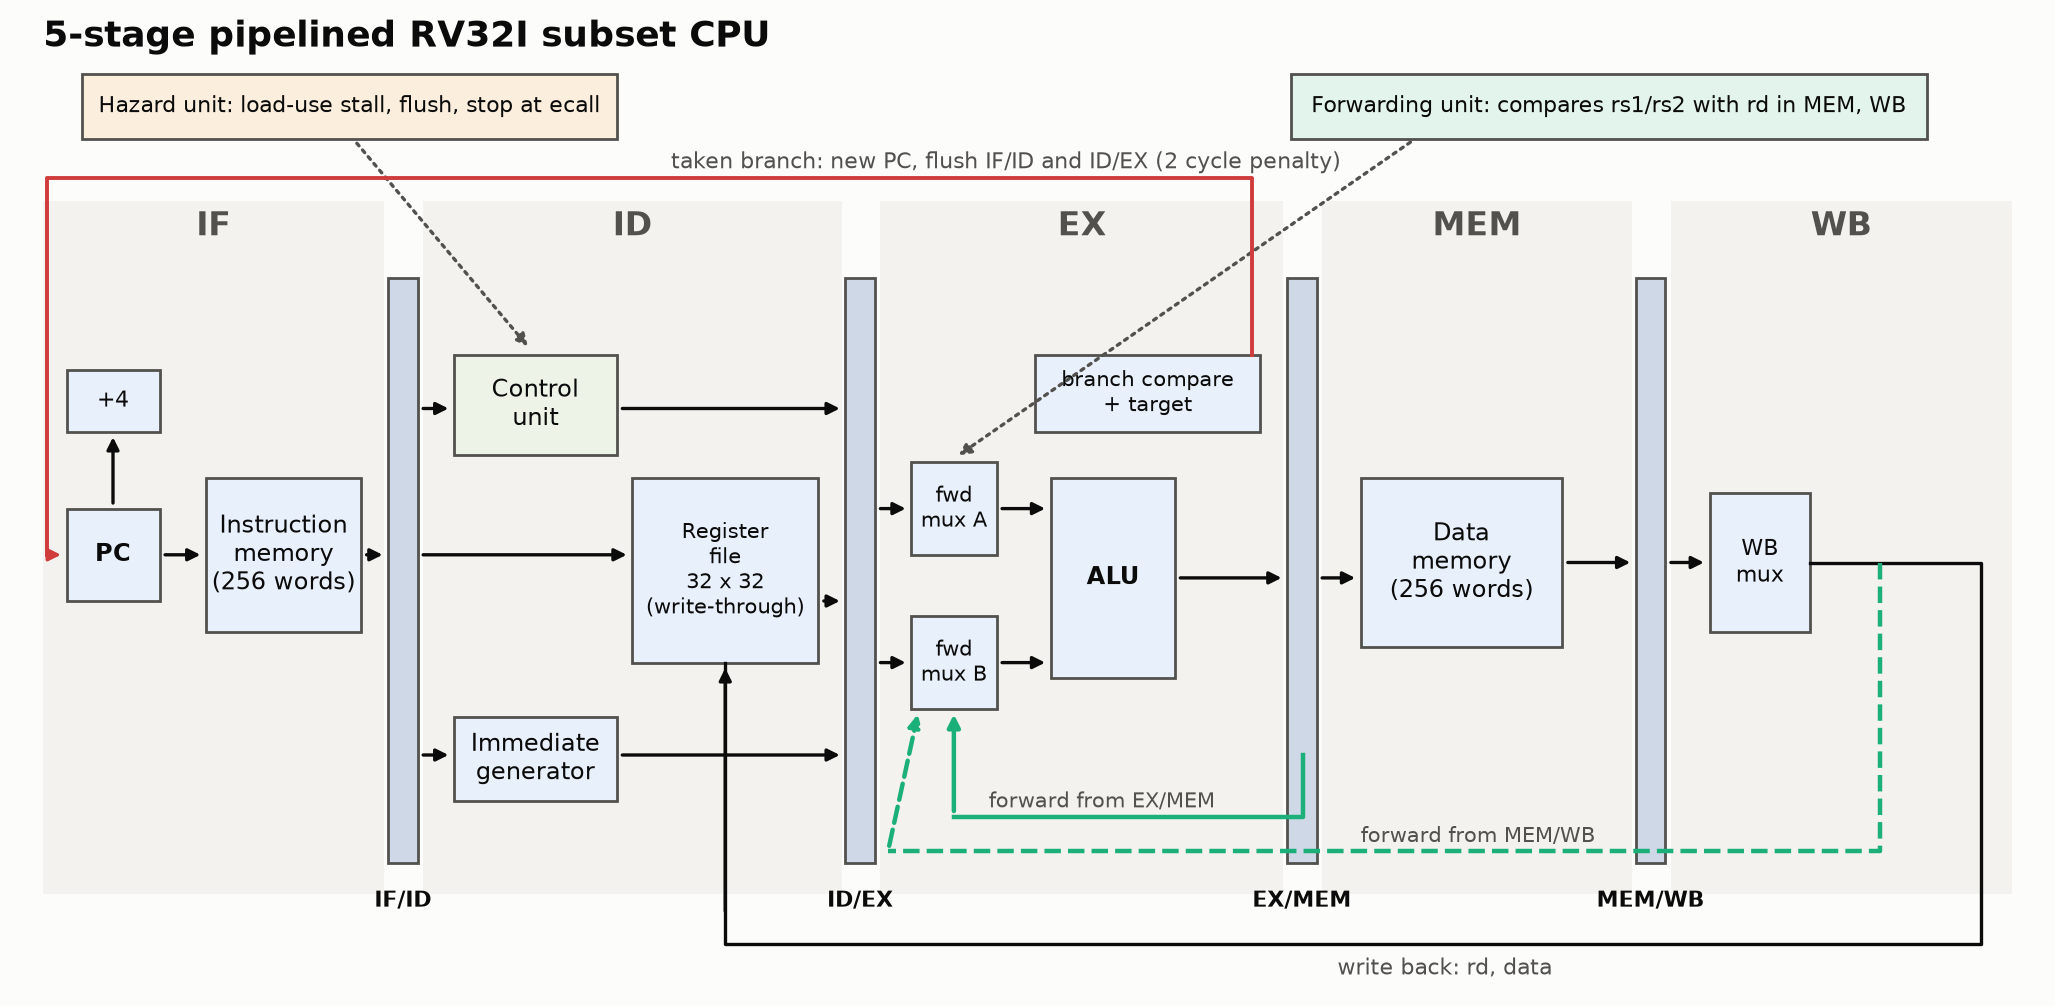
\includegraphics[width=\textwidth]{architecture_pipeline.png}
\caption{Datapath of the pipelined CPU. Grey bars are pipeline registers.
Green paths forward results to the ALU inputs; the red path redirects the PC
and flushes the two younger instructions on a taken branch.}
\label{fig:arch}
\end{figure*}

\subsection{Partitioning}
We cut the verified single-cycle datapath at four points
(Fig.~\ref{fig:arch}), one Verilog module per stage and per pipeline register,
following the brief: \texttt{if\_stage} (PC and instruction memory),
\texttt{id\_stage} (control unit, immediate generator and register file),
\texttt{ex\_stage} (forwarding muxes, ALU, branch comparator and target),
\texttt{mem\_stage} (data memory) and \texttt{wb\_stage} (write-back mux).
\texttt{cpu\_pipeline.v} only wires them together. Datapath and control are
partitioned the same way: control signals are decoded once in ID and travel
with their instruction through the pipeline registers, and each stage uses
only the signals it needs.

\subsection{Pipeline registers}
Table~\ref{tab:pregs} lists what each register carries. Every register
holds a \texttt{valid} bit, so a bubble is an ordinary entry with
\texttt{valid}=0 and all control bits zero. The PC travels with each
instruction because EX needs it for the branch target; the copies in later
stages exist for tracing and are removed by synthesis.

\begin{table}[t]
\centering
\caption{Pipeline register contents}
\label{tab:pregs}
\begin{tabular}{@{}lp{5.3cm}@{}}
\toprule
Register & Fields \\
\midrule
IF/ID & valid, PC, instruction \\
ID/EX & valid, PC, rs1 and rs2 values, immediate, rs1, rs2 and rd numbers,
RegWrite, ALUSrc, MemRead, MemWrite, Branch, BranchNe, Halt, ALU op \\
EX/MEM & valid, PC, ALU result, store data, rd, RegWrite, MemRead, MemWrite,
Halt \\
MEM/WB & valid, PC, ALU result, loaded word, rd, RegWrite, MemRead, Halt \\
\bottomrule
\end{tabular}
\end{table}

A flush clears only \texttt{valid} and the control bits, as in the textbook
design \cite{patterson2021}; data fields of a bubble are never used. Our first
version also cleared every data field. That put a synchronous reset on about
140 flip-flops at the end of the branch flush path, the slowest path of the
forwarding pipeline. Clearing control only raised its Fmax from 76.2 to
83.9\,MHz with no change in behaviour.

\subsection{Register file timing}
The register file is written at the end of WB and read in ID. When an
instruction in ID reads the register that WB is writing in the same cycle,
the register file returns the value being written (write-through). This is the
hardware form of the textbook ``write in the first half, read in the second
half'', and it removes the hazard at distance three without any forwarding
path. The single-cycle CPU must not have this bypass: there the write data
depends on the read data, and the bypass mux forms a combinational loop, which
Yosys reported on our first synthesis run. A Verilog \texttt{generate} block
builds the bypass only when the parameter asks for it.

\subsection{Forwarding unit}
For each ALU operand the forwarding unit compares the source register of the
instruction in EX with the destination of the instructions in MEM and WB:
\begin{equation*}
\mathit{fwdA} =
\begin{cases}
\text{EX/MEM} & \text{if } \mathit{RegWrite}_{M} \wedge rd_{M} = rs1_{E},\\
\text{MEM/WB} & \text{else if } \mathit{RegWrite}_{W} \wedge rd_{W} = rs1_{E},\\
\text{register file} & \text{otherwise,}
\end{cases}
\end{equation*}
and the same for operand B with $rs2_{E}$. EX/MEM wins because it holds the
newer value when both match. \textit{RegWrite} is already 0 when $rd$ is
x0, so a write to x0 is never forwarded. The forwarded operand B is also the
store data, so a store can save a value computed by the instruction just
before it. Setting the parameter \texttt{FORWARDING} to 0 ties both selects
to ``register file'', which gives the second pipeline in our comparison.

\subsection{Hazard unit}
With forwarding, the only data hazard that must stall is a load followed
at once by a use of its result:
\begin{align*}
\mathit{loadUse} = {} & \mathit{MemRead}_{E} \wedge \mathit{RegWrite}_{E} \\
& \wedge \big( (\mathit{usesRs1}_{D} \wedge rs1_{D} = rd_{E}) \\
& \quad \vee (\mathit{usesRs2}_{D} \wedge rs2_{D} = rd_{E}) \big).
\end{align*}
The \textit{usesRs} flags come from the control unit, so immediate bits that
look like a register number never cause a stall. Without forwarding, the unit stalls whenever the
instruction in ID reads the destination of the instruction in EX or MEM.
A stall holds the PC and IF/ID and turns ID/EX into a bubble.

A taken branch is resolved in EX. The PC loads the target, and IF/ID and
ID/EX are flushed, which discards the two instructions fetched on the wrong
path. A flush takes priority over a stall, because the stalled instruction
is itself on the wrong path.

\subsection{Stopping at \texttt{ecall}}
The pipeline fetches instructions behind \texttt{ecall} before it reaches
WB, and a store among them would change memory. When \texttt{ecall} leaves
ID (and is not being flushed), the hazard unit freezes the PC and feeds
bubbles into IF/ID from then on. The program ends when \texttt{ecall}
reaches WB, after every older instruction has completed.

% ABOUTME: Verification: the ISS reference model, directed and random tests, counters, bugs found.
% ABOUTME: Owner: Trishit (review, add annotated waveform screenshots from GTKWave or Surfer).
\section{Verification}
\label{sec:verification}

\subsection{Method}
A test passes only if the hardware ends in exactly the state the
instruction set architecture defines. We wrote a two-pass assembler and an
instruction set simulator (ISS) in Python (\texttt{tools/rvasm.py},
\texttt{tools/iss.py}). The assembler's encodings are checked against the
RISC-V specification \cite{riscvspec} by 34 unit tests, and the ISS is checked
on hand-computed programs before anything is compared with it. One
testbench (\texttt{tb/tb\_cpu.v}) serves all three CPUs under Icarus Verilog
\cite{icarus}. It runs a program until \texttt{ecall}, then dumps all 32
registers, all 256 data words and the performance counters. The runner
(\texttt{tools/sim.py}) compares every register, every memory word and the
instruction count with the ISS. Each program runs on all three CPUs.

\subsection{Tests}
Directed tests (Table~\ref{tab:tests}) each aim at one case the pipeline can
get wrong. Five benchmarks (array sum, Fibonacci, bubble sort and two
microbenchmarks) are checked the same way. A constrained-random generator
(\texttt{tools/randprog.py}) writes 40 programs of 46 instructions over only
six registers, mixing arithmetic, loads and stores to eight shared words and
forward branches, so hazards at every distance occur far more often than in
hand-written code. Finally, four tests check the performance counters: CPI is
exactly 1 on the single-cycle CPU, (\ref{eq:cycles}) holds on every program, a
false hazard costs no cycle, and forwarding leaves no arithmetic stall.
In total the suite runs 229 checks in about three seconds and runs in
continuous integration on every pull request.

\begin{table}[t]
\centering
\caption{Directed tests}
\label{tab:tests}
\begin{tabular}{@{}lp{5.4cm}@{}}
\toprule
Program & What it catches \\
\midrule
\texttt{alu\_ops} & every ALU operation, signed compares, shift by 31 \\
\texttt{x0\_reg} & writes to x0 dropped, never forwarded \\
\texttt{raw\_hazards} & RAW at distance 1, 2 and 3 on both operands \\
\texttt{load\_use} & load then use as rs1, rs2, base address, store data \\
\texttt{store\_data} & store data and address from the previous instruction \\
\texttt{branches} & taken and not taken, operands from ALU and load, back to back \\
\texttt{halt\_shadow} & instructions after \texttt{ecall} never commit \\
\texttt{false\_hazard} & immediate bits that look like rs2 do not stall \\
\texttt{hazard\_demo} & one forward, one load-use stall, one flush \\
\bottomrule
\end{tabular}
\end{table}

\subsection{Pipeline timing}
The testbench writes the PC in every stage on every cycle. From that trace we
draw the pipeline diagram of Fig.~\ref{fig:diagram}, so the figure shows the
hardware's behaviour, not our intention. Fig.~\ref{fig:wave} shows the same
run as a waveform, read from the simulation's VCD file. The overlap of
instructions, the stall of \texttt{add x4} behind the load, the two flushed
instructions after the taken \texttt{beq}, and the forwarding selects
(EX/MEM in cycles 4, 6 and 8, MEM/WB in cycle 7) are all visible.

\begin{figure}[t]
\centering
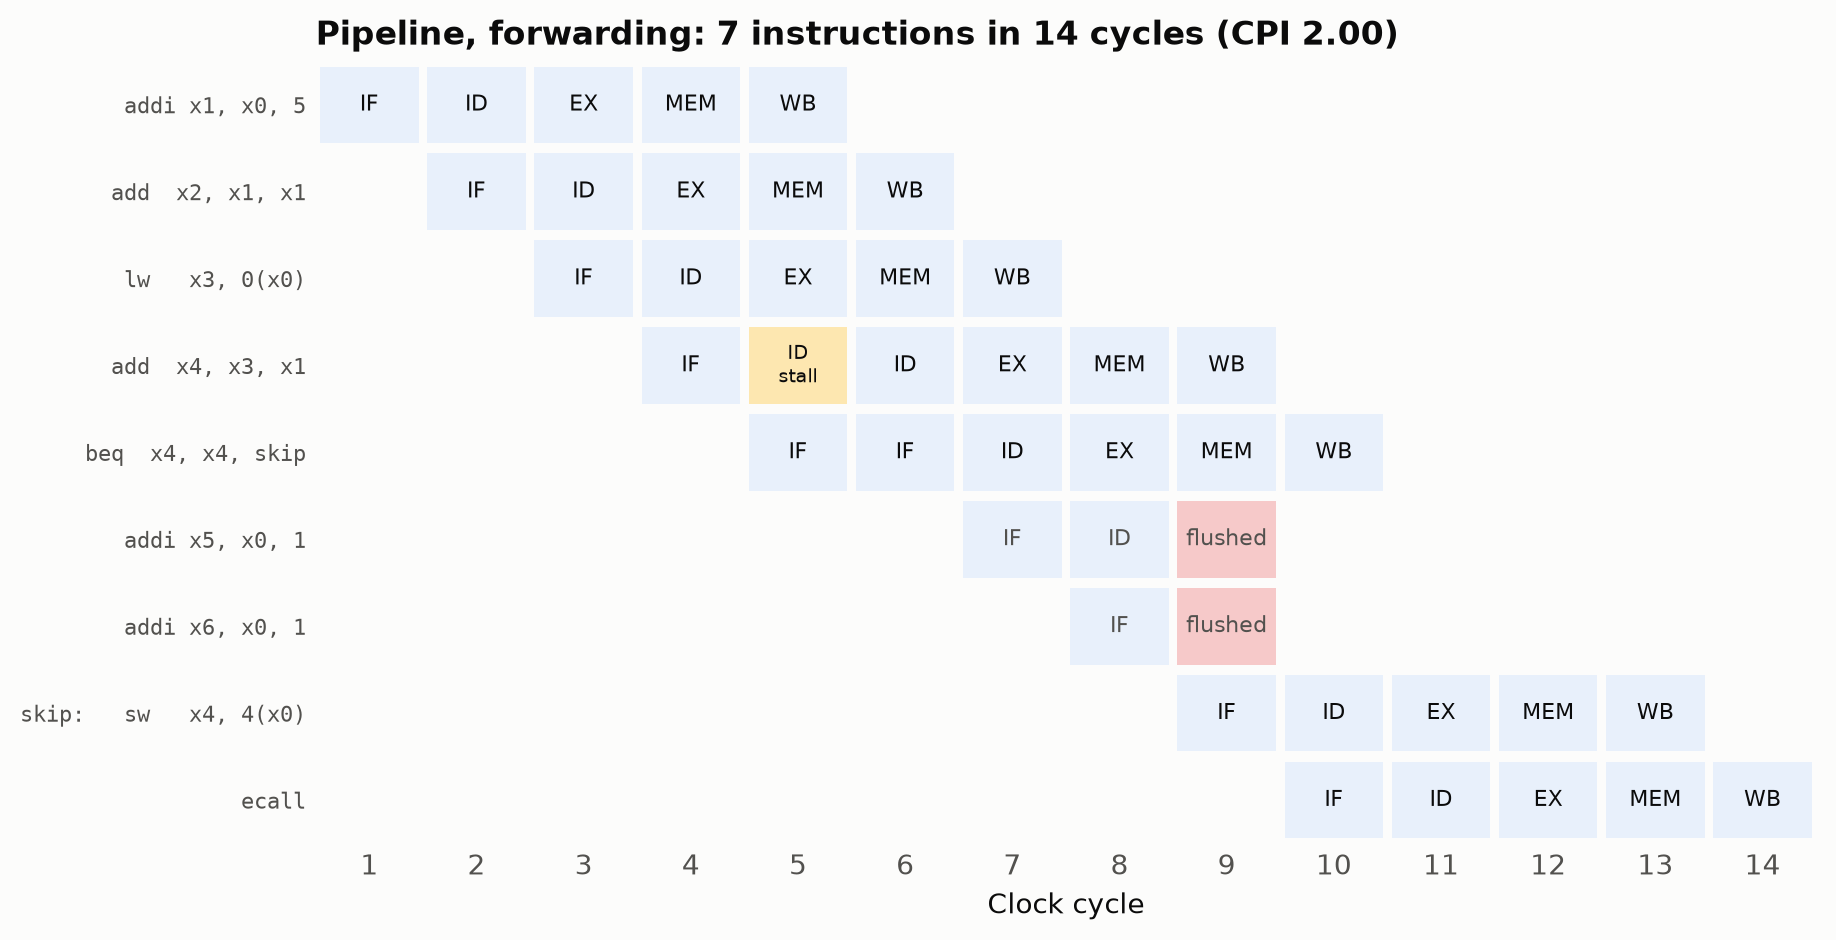
\includegraphics[width=\columnwidth]{pipeline_diagram_pipe_fwd.png}
\caption{Pipeline diagram of the hazard demo on the forwarding pipeline,
drawn from the RTL trace. Yellow: load-use stall. Red: flushed.}
\label{fig:diagram}
\end{figure}

\begin{figure}[t]
\centering
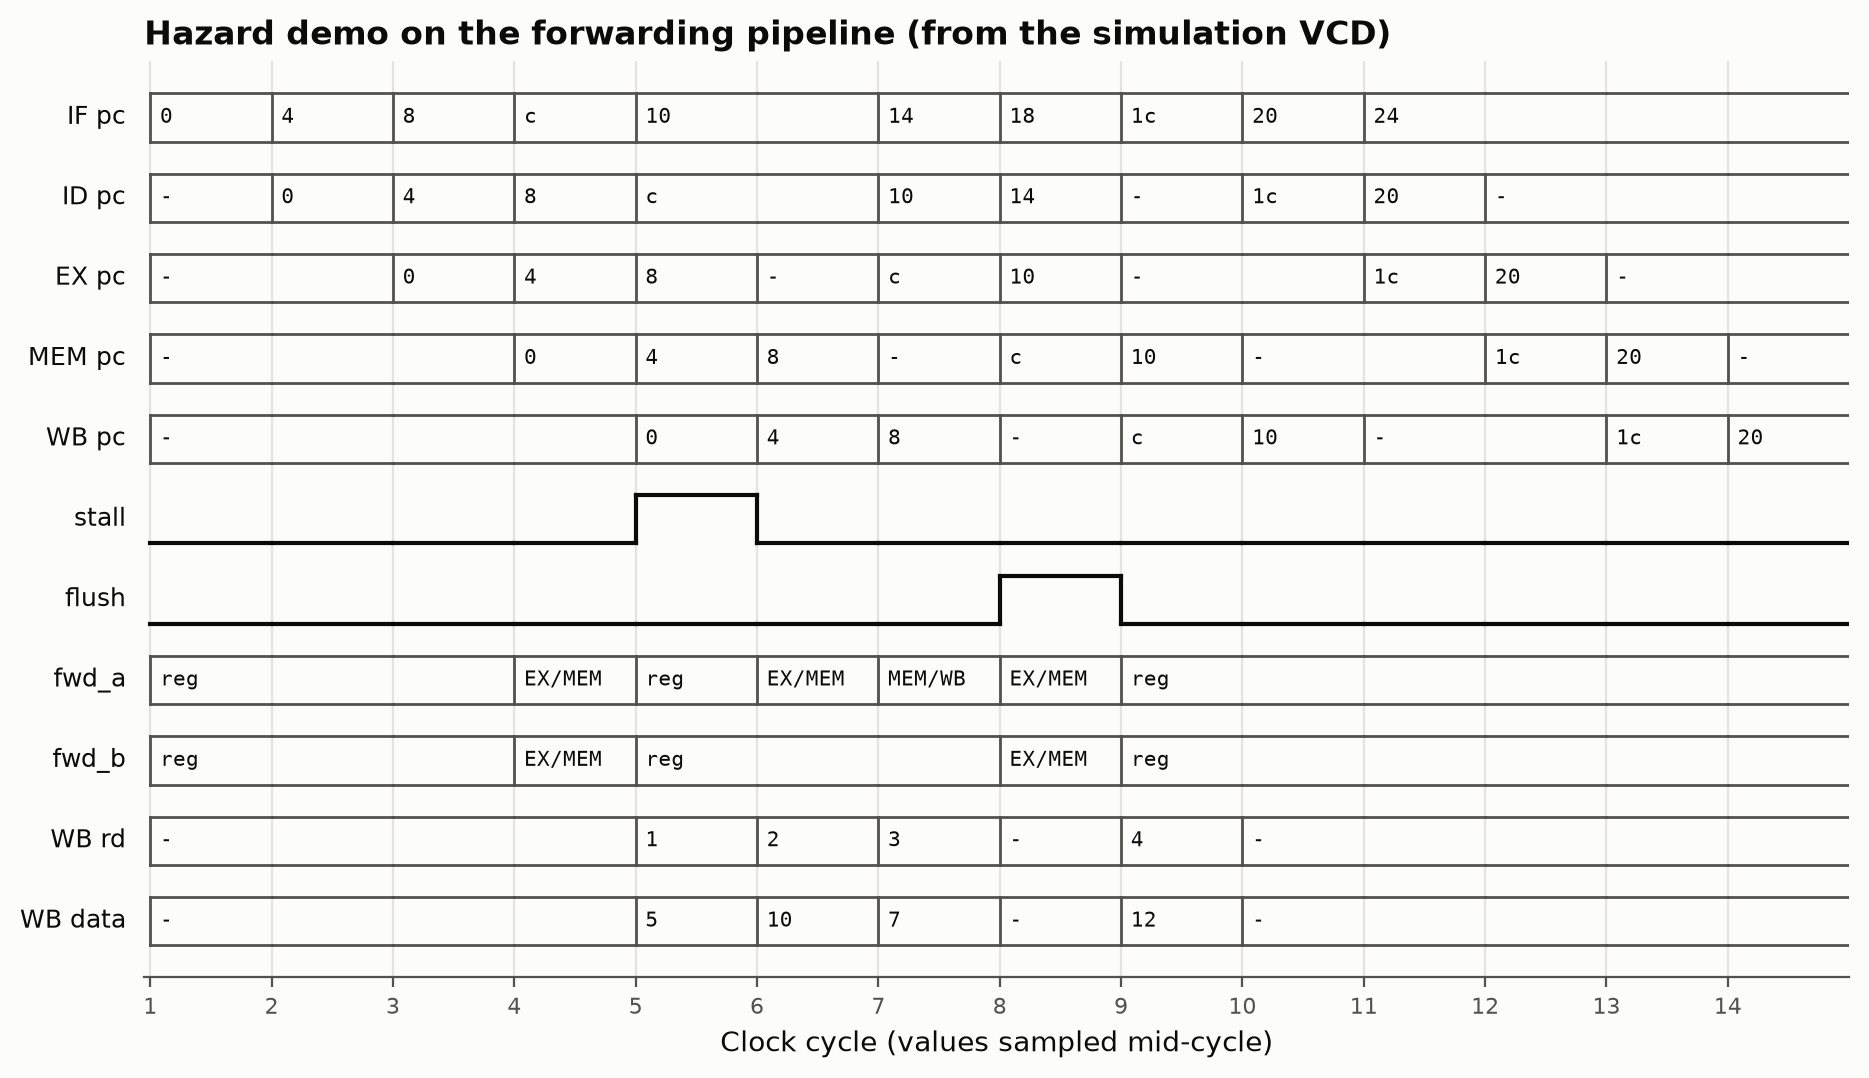
\includegraphics[width=\columnwidth]{waveform_hazard_demo.png}
\caption{Waveform of the same run: PC in each stage (\texttt{-} is a bubble),
stall, flush, forwarding selects and write back.}
\label{fig:wave}
\end{figure}

\subsection{Bugs the flow caught}
Four defects were found and fixed during development, each with its root
cause:
\begin{enumerate}
\item The forwarding and hazard logic was first written as Verilog functions
called from \texttt{assign}. Such an assignment is only re-evaluated when the
function's \emph{arguments} change, not when the module signals it reads
change, so forwarding selects went stale. The ISS comparison failed on the
first program; the logic now uses \texttt{always @(*)}.
\item With forwarding disabled, Icarus folded the constant \texttt{if
(ENABLE)} away and left an \texttt{always @(*)} block with no sensitivity,
so the selects stayed unknown. The enable now applies outside the block.
\item Synthesis of the single-cycle CPU reported a combinational loop through
the register file bypass (Section~\ref{sec:pipeline}).
\item An initial NOP fill of instruction memory took priority over the
program file in one synthesis mode, so Yosys saw a CPU that only ran NOPs and
removed it entirely. The fill now exists only in simulation.
\end{enumerate}

% Keep the verification evidence before Results, including full-width floats.
\clearpage
% ABOUTME: Results: synthesis, CPI and IPC, execution time, and why the speedup is what it is.
% ABOUTME: Owner: Husain (review every number against results/, rerun make synth perf to check).
\section{Results}
\label{sec:results}

\subsection{Setup}
Synthesis uses Yosys \cite{yosys} (\texttt{synth\_ecp5}) and place and route
uses nextpnr \cite{nextpnr} for a Lattice ECP5 LFE5U-25F, speed grade 6,
package CABGA381 \cite{ecp5}, the FPGA on boards such as the ULX3S. Each CPU
sits in a small top level that shows the last value written back on eight
LEDs, so no logic can be optimised away, and runs the bubble sort program from
its instruction ROM. nextpnr results depend on a random placement seed, so
each design is placed with five seeds and we report the median.

\subsection{Synthesis}
Table~\ref{tab:synth} gives the results. The pipeline registers add about
260 flip-flops. Without forwarding the pipeline's clock is 1.94 times the
single-cycle clock; with forwarding it is 1.43 times, because the forwarding
comparators and muxes sit in front of the ALU and the branch comparator, on
the path that ends in the flush of IF/ID and ID/EX.

\begin{table}[t]
\centering
\caption{ECP5 results, median of five seeds (LUT memories)}
\label{tab:synth}
\small
\setlength{\tabcolsep}{3pt}
\begin{tabular}{@{}lrrrr@{}}
\toprule
CPU & Logic cells & FFs & Fmax (MHz) & Range \\
\midrule
Single-cycle & 2076 & 43 & 58.75 & 57.7--60.2 \\
Pipeline, no fwd & 2137 & 299 & 113.86 & 110.1--115.5 \\
Pipeline, fwd & 2765 & 308 & 83.89 & 83.6--86.9 \\
\bottomrule
\end{tabular}
\end{table}

\textbf{Memory style matters.} When Yosys may use the FPGA's block RAM, it
notices that each memory feeds a pipeline register and folds that register
into the block RAM. This is legal and saves flip-flops, but an ECP5 block RAM
has a 5.6\,ns clock-to-output delay, so the ID stage and the MEM/WB forwarding
path then start with 5.6\,ns already spent. With block RAM the three designs
reach only 42.2, 72.2 and 59.1\,MHz (Fig.~\ref{fig:fmax}). We therefore place
both 256 word memories in LUTs, where every pipeline register stays a real
flip-flop and the stage boundaries in the RTL are the stage boundaries in the
hardware. Larger memories would need block RAM and an extra pipeline stage or a
registered address, as real processors do.

\begin{figure}[t]
\centering
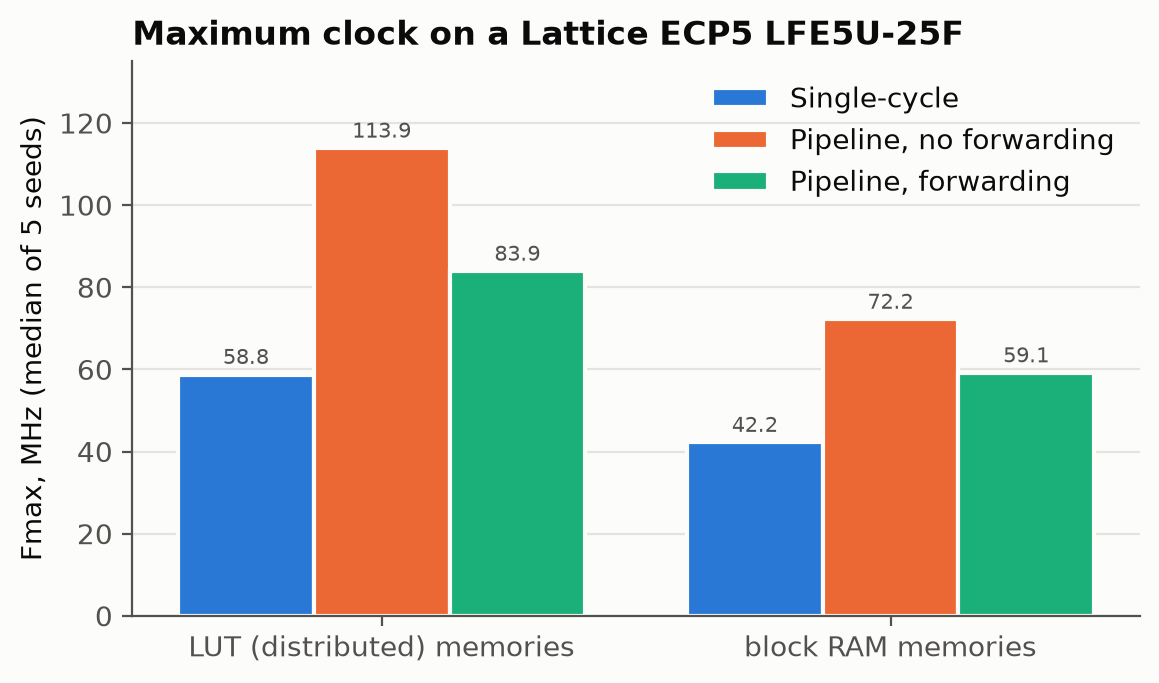
\includegraphics[width=\columnwidth]{fmax.png}
\caption{Fmax of each CPU with LUT memories and with block RAM.}
\label{fig:fmax}
\end{figure}

\subsection{CPI and IPC}
Table~\ref{tab:cpi} lists CPI and IPC for every benchmark. The single-cycle
CPU has CPI 1.00 by construction. Fig.~\ref{fig:breakdown} splits each
pipelined CPI with (\ref{eq:cycles}). Without forwarding, data hazard stalls
dominate: \texttt{dep\_chain}, where each instruction needs the one before
it, stalls for 241 cycles over 163 instructions. Forwarding removes every
one of those stalls; what remains are load-use stalls (66 in bubble sort, one
per inner iteration, and 16 in the array sum) and branch flushes. Every loop
iteration ends in a taken branch, so with loop bodies of six to ten
instructions the flushes alone add 0.23 to 0.35 to CPI. The four fill cycles
are negligible for programs of 86 instructions or more.

\begin{table}[t]
\centering
\caption{CPI (IPC in brackets) per benchmark}
\label{tab:cpi}
\small
\setlength{\tabcolsep}{4pt}
\begin{tabular}{@{}lrrr@{}}
\toprule
Benchmark ($N$) & Single & Pipe, no fwd & Pipe, fwd \\
\midrule
bubble\_sort (591) & 1.00 & 2.07 (0.48) & 1.45 (0.69) \\
dep\_chain (163) & 1.00 & 2.74 (0.37) & 1.26 (0.80) \\
fibonacci (215) & 1.00 & 1.71 (0.59) & 1.29 (0.78) \\
indep\_ops (162) & 1.00 & 1.51 (0.66) & 1.26 (0.79) \\
sum\_array (86) & 1.00 & 2.16 (0.46) & 1.58 (0.63) \\
\bottomrule
\end{tabular}
\end{table}

\begin{figure*}[t]
\centering
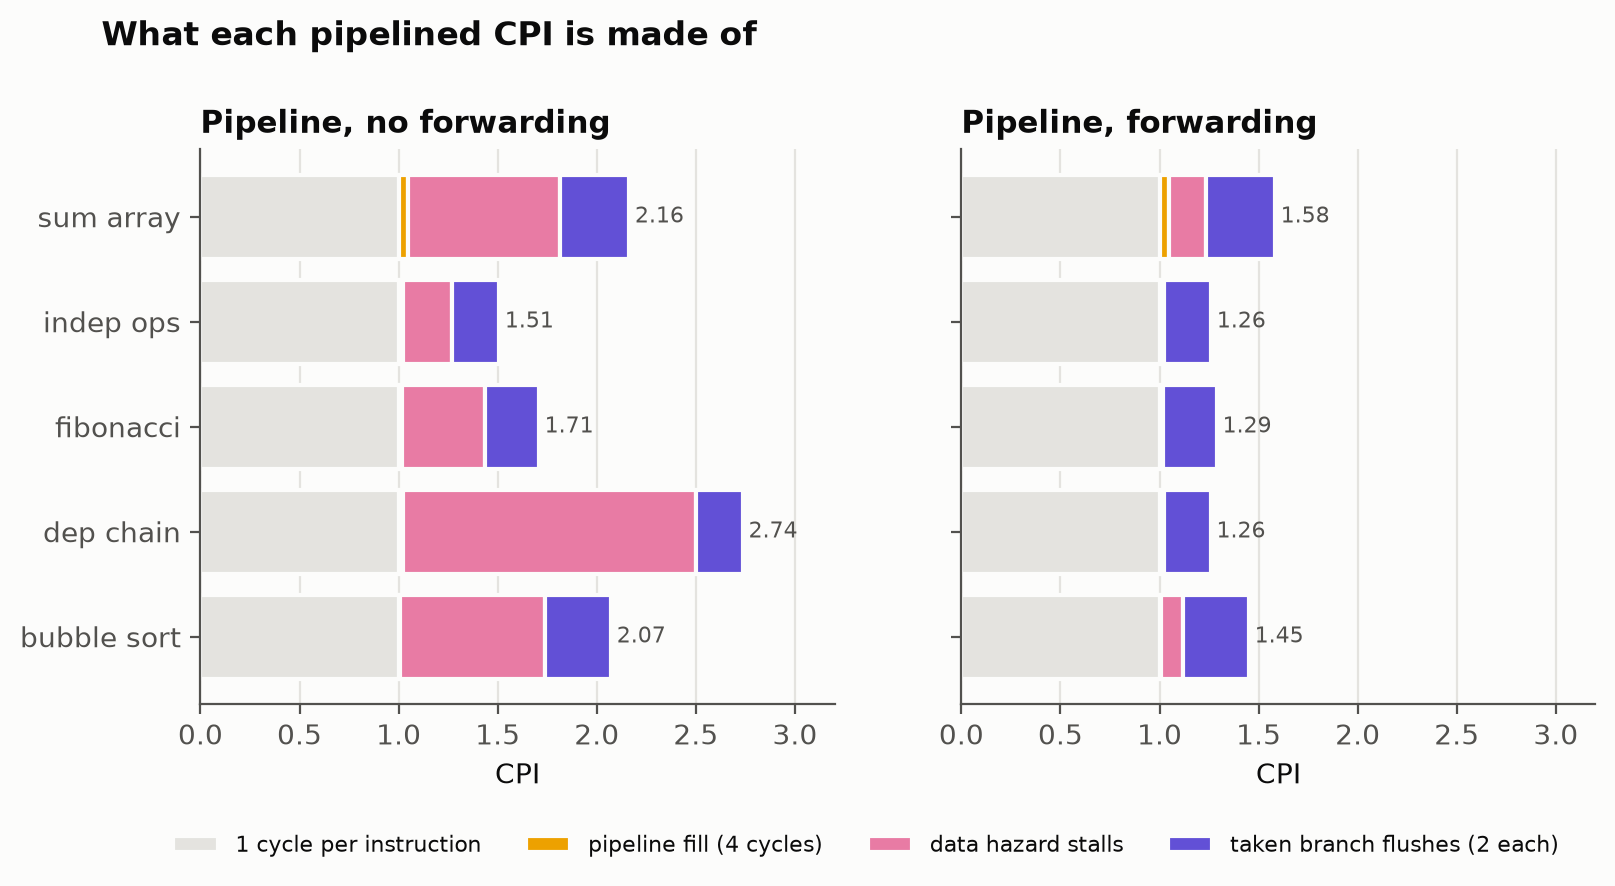
\includegraphics[width=0.85\textwidth]{cpi_breakdown.png}
\caption{Where the pipelined cycles go: one cycle per instruction plus fill,
data hazard stalls and taken branch flushes, per benchmark.}
\label{fig:breakdown}
\end{figure*}

\subsection{Execution time}
Combining cycles with Fmax gives execution time and the speedup over the
single-cycle CPU (Fig.~\ref{fig:speedup}). Equation (\ref{eq:speedup}) makes
the outcome predictable: the forwarding pipeline wins only when its CPI is
below 1.43, and the pipeline without forwarding only when its CPI is below
1.94. With forwarding, \texttt{dep\_chain}, \texttt{fibonacci} and
\texttt{indep\_ops} (CPI 1.26 to 1.29) run 1.11 to 1.14 times faster, while
bubble sort and the array sum (CPI 1.45 and 1.58) run slightly slower. The
pipeline without forwarding has the best clock and wins on code with few
dependences (\texttt{indep\_ops}, 1.29 times), but loses badly on dependent
chains (0.71 times). Forwarding therefore trades a 26\,\% slower clock for a
much more predictable CPI: its worst case is 0.90, against 0.71 without it.

\begin{figure}[t]
\centering
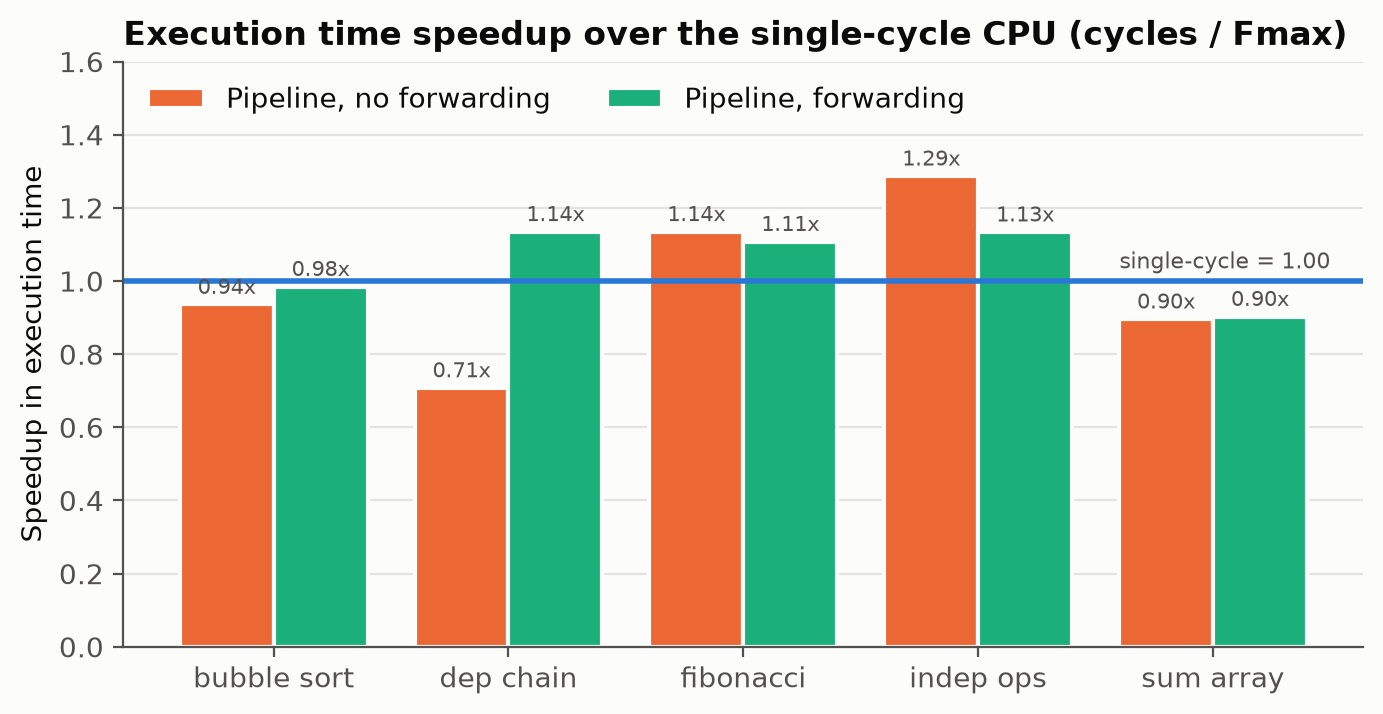
\includegraphics[width=\columnwidth]{speedup.png}
\caption{Execution time speedup over the single-cycle CPU (cycles divided by
Fmax). Above 1 the pipeline is faster.}
\label{fig:speedup}
\end{figure}

\subsection{Why not five times faster}
An ideal five-stage pipeline would have a clock five times faster and
CPI 1. Ours falls short on both counts. First, the stages are not balanced:
the data memory read alone takes 8.0 of the single-cycle CPU's 17.0\,ns, and
EX holds the ALU, the forwarding muxes and the branch decision, so the
longest stage is about half of the single-cycle path, not a fifth. Second,
the branch penalty of two cycles per loop iteration costs a quarter to a
third of a cycle per instruction. The clearest next steps are therefore a
branch predictor or resolving branches in ID (one cycle penalty instead of
two), and rebalancing the slowest stages: EX, whose ALU and forwarding path
set the clock in both pipelines, and MEM, whose 8\,ns memory read is close
behind.

% ABOUTME: Conclusion: what Phase I built and measured, where the project stands, and the Phase II plan.
% ABOUTME: Owner: Navodit. Every number here is from results/ (cpi.csv, performance.csv, synth.csv).
\section{Conclusion, Current Progress and Phase II Plan}
\label{sec:conclusion}

\subsection{Conclusion}
We built three processors for the same RV32I subset: a single-cycle CPU and
a five-stage pipeline with and without forwarding. Pipelining raised the
clock 1.94 times without forwarding and 1.43 times with it, but CPI rose to
1.51 to 2.74 and 1.26 to 1.58, so the net speedup ranged from 0.71 to 1.29.
The iron law explains each of these numbers: a pipeline is faster only when
the clock it gains is larger than the CPI it loses. In our programs the
largest single loss is the two-cycle flush after every taken branch, because
every loop iteration ends in one.

\subsection{Current progress}
Phase I is complete. All three CPUs are written in Verilog and pass all 248
automated checks against the reference simulator. They are synthesised and
placed for a Lattice ECP5 FPGA, and the CPI and speedup study is done. Every
table and figure in this report is generated from the repository by
\texttt{make synth perf figures}, so any change in Phase II can be measured
the same way.

\subsection{Phase II plan}
Phase II targets the two losses this report measures.
\begin{enumerate}
\item \emph{Branches.} Taken branch flushes add 0.23 to 0.35 to CPI. We will
first resolve branches in ID, which cuts the penalty to one cycle at the cost
of a comparator and forwarding paths in ID. Then we will add a dynamic
predictor with two-bit counters and a branch target buffer \cite{smith1981},
so a correctly predicted loop branch costs no cycles.
\item \emph{Stage balance.} EX is the longest stage in both pipelines (8.8 and
11.9\,ns). We will split it or move the branch decision out of it, so the
forwarding pipeline keeps more of its clock gain.
\item \emph{Instruction set.} Adding \texttt{jal}, \texttt{jalr} and byte and
halfword loads will let us run compiled C programs instead of hand-written
assembly.
\item \emph{Hardware.} We will run the design on a real ECP5 board using the
existing FPGA top level.
\end{enumerate}
Each change will be checked against the reference simulator and measured
with the same CPI and Fmax flow, so its gain can be compared directly with
the Phase I numbers.
% ABOUTME: Contributions section: who did what. Each member corrects their own entry.
% ABOUTME: Matches the owners in ROADMAP.md; update both if the split changes.
\section{Contributions}
\label{sec:contributions}

\begin{itemize}
\item \textbf{Sarvesh Srinath}: repository, RTL of both CPUs, hazard and
forwarding units, assembler, reference model, verification flow, synthesis
scripts and performance study; review and merging. Wrote
Section~\ref{sec:pipeline}.
\item \textbf{Aryan Kumar}: review of the datapath and control unit against
the RISC-V specification; the single-cycle design. Wrote
Section~\ref{sec:single}.
\item \textbf{Trishit Swarnakar}: verification review, additional directed
tests and annotated waveforms. Wrote Section~\ref{sec:verification}.
\item \textbf{Husain Khorakiwala}: reproduction of the synthesis and
performance results, analysis of the critical paths; review and merging,
and the final report build and submission, taken over from Sarvesh. Wrote
Section~\ref{sec:results}.
\item \textbf{Navodit Sharma}: background and related work, report assembly
and presentation slides. Wrote the abstract and Sections~\ref{sec:intro},
\ref{sec:background} and~\ref{sec:conclusion}.
\end{itemize}


\bibliographystyle{IEEEtran}
\bibliography{refs}

\end{document}
